\documentclass[12pt]{article}
\usepackage[utf8]{inputenc}

\usepackage{enumitem}
\usepackage[margin=2cm]{geometry}

\usepackage{amsmath, amsfonts, amssymb}
\usepackage{graphicx}
\usepackage{tikz}
\usepackage{pgfplots}
\usepackage{multicol}

\usepackage{comment}
\usepackage{url}
\usepackage{calc}
\usepackage{subcaption}

\usepackage{array}

\setlength\parindent{0pt}

\usepackage{fancyhdr}
\pagestyle{fancy}
\fancyhf{}
\renewcommand{\headrulewidth}{2pt}
\renewcommand{\footrulewidth}{0pt}
\rfoot{\thepage}
\lhead{\textsc{Math} 244}
\chead{\textsc{Homework 2}}
\rhead{Fall 2023}

\pgfplotsset{compat=1.16}

% MATH commands
\newcommand{\ga}{\left\langle}
\newcommand{\da}{\right\rangle}
\newcommand{\oa}{\left\lbrace}
\newcommand{\fa}{\right\rbrace}
\newcommand{\oc}{\left[}
\newcommand{\fc}{\right]}
\newcommand{\op}{\left(}
\newcommand{\fp}{\right)}

\newcommand{\bi}{\mathbf{i}}
\newcommand{\bj}{\mathbf{j}}
\newcommand{\bk}{\mathbf{k}}
\newcommand{\bF}{\mathbf{F}}

\newcommand{\ra}{\rightarrow}
\newcommand{\Ra}{\Rightarrow}

\newcommand{\sech}{\mathrm{sech}\,}
\newcommand{\csch}{\mathrm{csch}\,}
\newcommand{\curl}{\mathrm{curl}\,}
\newcommand{\dive}{\mathrm{div}\,}

\newcommand{\ve}{\varepsilon}
\newcommand{\spc}{\vspace*{0.5cm}}

\DeclareMathOperator{\Ran}{Ran}
\DeclareMathOperator{\Dom}{Dom}

\newcommand{\exo}[3]{\noindent\textcolor{red}{\fbox{\textbf{Section {#1}, Problem {#2}}}\hrulefill   \textbf{({#3} Pts})}\vspace*{10pt}}

\begin{document}
\thispagestyle{empty}
	\noindent \hrulefill \newline
	MATH-244 \hfill Pierre-Olivier Paris{\'e}\newline
	Homework 2 Solutions \hfill Fall 2023\newline \vspace*{-0.7cm}
	
	\noindent\hrulefill
	
	\spc
	
	\exo{15.2}{8}{5}
	
	The region $D$ is a type II domain, with $h_1 (x) = y-1$ and $h_2 (x) = 1$. See the picture below.
		\begin{center}
		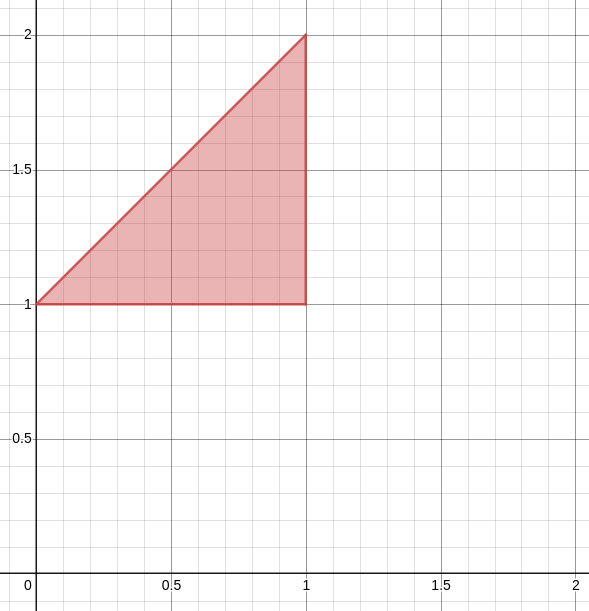
\includegraphics[scale=0.5]{DomainExo8.png}
		\end{center}
	from the formula,
		\begin{align*}
		\iint_D (2x + y) \, dA &= \int_1^2 \int_{y - 1}^1 2x + y \, dx dy \\
		&= \int_1^2 \left. (x^2 + xy) \right|_{y-1}^1 \, dy \\
		&= \int_1^2 1 + y - \Big( (y-1)^2 + (y-1) y \Big) \, dy \\
		&= \int_1^2 1 + y - y^2 + 2y - 1 - y^2 + y \, dy \\
		&= \int_1^2 4y - 2y^2 \, dy \\
		&= \left. ( 2y^2 - (2/3) y^3 ) \right|_1^2 = 4/3 .
		\end{align*} 
	The answer should therefore by $4/3$.

	\exo{15.2}{12b}{5}

	Here is an example of a region $D$ which is neither of Type I nor of Type II.
	\begin{center}
	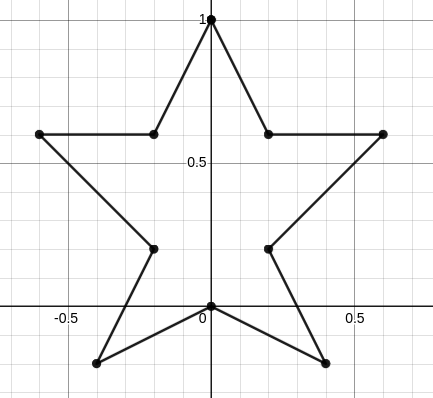
\includegraphics[scale=0.5]{NonTypeITypeIIRegion.png}
	\end{center}

	\exo{15.2}{16}{10}

	The region is illustrated below.
	\begin{center}
	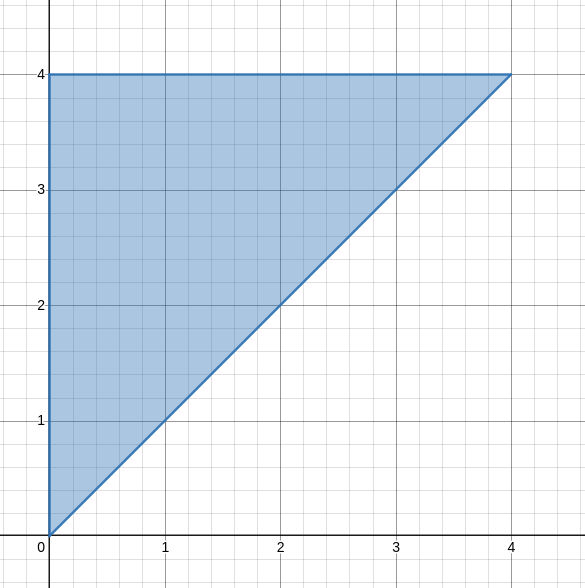
\includegraphics[scale=0.5]{Exercise16Region.png}
	\end{center}


	\underline{\textbf{Type I}.} To integrate firstly in $y$ (inner integral) and secondly in $x$ (outer integral), we need to give a description of $D$. We have
		\begin{align*}
		D = \{ (x, y) \, : \, 0 \leq x \leq 4 \text{ and } x \leq y \leq 4 \} .
		\end{align*}
	Therefore,
		\begin{align*}
		\iint_D y^2 e^{xy} \, dA = \int_0^4 \int_x^4 y^2 e^{xy} \, dy dx .
		\end{align*} 
	But this integral is hard because, after integrating by parts two times, we get
		\begin{align*}
		\iint_D y^2 e^{xy} \, dA = \int_0^4 \left. \Big( \frac{y^2 e^{xy}}{x} - \frac{2y e^{xy}}{x^2} + \frac{2 e^{xy}}{x^3} \Big) \right|_x^4 \, dx .
		\end{align*} 
	This is really hard to integrate! We instead consider the region as a Type II. \vspace*{12pt}

	\underline{\textbf{Type II}.} The description of the region as a type II is
		\begin{align*}
		D = \{ (x, y) \, : \, 0 \leq x \leq y \text{ and } 0 \leq y \leq 4 \}.
		\end{align*} 
	Therefore,
		\begin{align*}
		\iint_D y^2 e^{xy} \, dA &= \int_0^4 \int_0^y y^2 e^{xy} \, dx dy \\
		&= \int_0^4 \left. ye^{xy} \right|_0^y \, dy \\
		&= \int_0^4 ye^{y^2} - y \, dy \\
		&= \left. \Big( \frac{e^{y^2}}{2} - \frac{y^2}{2} \Big) \right|_0^4\\
		&= \frac{e^{16} - 17}{2} .
		\end{align*} 


	\exo{15.2}{26}{10}

	The domain $D$ is
		\begin{align*}
		D = \{ (x, y) \, : \, x \geq 0 , y \geq 0 , x + y = 2 \} .
		\end{align*}
	We will describe $D$ as a type I domain:
		\begin{align*}
		D = \{ (x, y) \, : \, 0 \leq x \leq 2 \text{ and } 0 \leq y \leq 2 - x \} .
		\end{align*} 
	Therefore,
		\begin{align*}
		Vol = \iint_D x^2 + y^2 + 1 \, dA & = \int_0^2 \int_0^{2-x} x^2 + y^2 + 1 \, dy dx \\
		&= \int_0^2 \left. \Big( x^2y + \frac{y^3}{3} + y \Big) \right|_0^{2-x} \, dx \\
		&= \int_0^2 x^2 (2-x) + \frac{(2 - x)^3}{3} + 2 - x \, dx \\
		&= \left. \Big( \frac{2x^3}{3} - \frac{x^4}{4} - \frac{(2 - x)^4}{12} + 2x - \frac{x^2}{2} \Big) \right|_0^2 \\
		&= \frac{14}{3} \approx 4.6667 .
		\end{align*}


	\exo{15.2}{46}{10}

	From the bounds in the iterated integral, we have
		\begin{align*}
		D = \{ (x, y) \, : \, 0 \leq x \leq 2 \text{ and } x^2 \leq y \leq 4 \} .
		\end{align*} 
	\begin{center}
		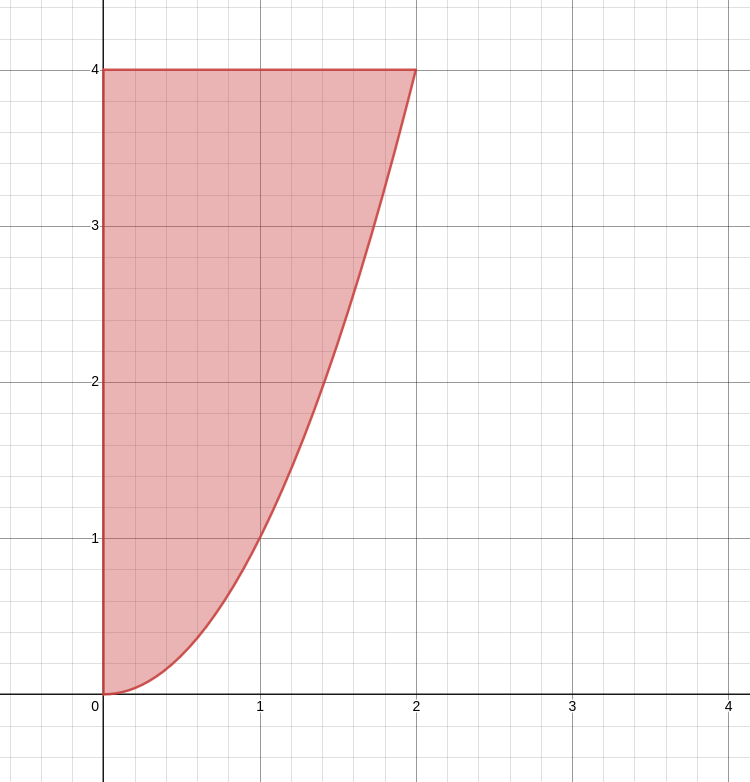
\includegraphics[scale=0.5]{Exo46RegionPicture.png}
	\end{center}

	From the picture, we see that $0 \leq y \leq 4$. The function acting as a lower-bound for the region is $y = x^2$, so that $\sqrt{y} = x$ because $x$ is positive when restricted to the region $D$. Therefore, 
		\begin{align*}
		D = \{ (x, y) \, : \, 0 \leq y \leq 4 \text{ and } 0 \leq x \leq \sqrt{y} \}. 
		\end{align*} 
	The integral then become
		\begin{align*}
		\int_0^2 \int_{x^2}^4 f (x, y) \, dy dx = \iint_D f (x,y) \, dA = \int_0^4 \int_0^{\sqrt{y}} f (x, y) \, dx dy .
		\end{align*} 


	\exo{15.2}{56}{10}

	From the bounds in the iterated integral, we have
		\begin{align*}
		D = \{ (x, y) \, : \, 0 \leq y \leq 8 \text{ and } \sqrt[3]{y} \leq x \leq 2 \} .
		\end{align*} 
	The lowerbound for $x$ is the function $x = \sqrt[3]{y}$, so that $x^3 = y$. So, when $y = 0$, we get $x = 0$ and when $y = 8$, we get $x = 2$. The description of $D$ as a type I is therefore
		\begin{align*}
		D = \{ (x ,y) \, : \, 0 \leq x \leq 2 \text{ and } 0 \leq y \leq x^3 \} .
		\end{align*} 

	The integral then becomes
		\begin{align*}
		\int_0^8 \int_{\sqrt[3]{y}}^2 e^{x^4} \, dx dy = \iint_D e^{x^4} \, dA &= \int_0^2 \int_0^{x^3} e^{x^4} \, dydx \\
		&= \int_0^2 (x^3 - 0) e^{x^4} \, dx \\
		&= \left. \Big( \frac{e^{x^4}}{4} \Big) \right|_0^2 \\
		&= \frac{e^{16} - 1}{4} .
		\end{align*} 


\end{document}